\subsection{Cronograma de actividades}
\label{sec:cronograma-actividades}

Este cronograma es la hoja de ruta que permite al equipo del proyecto mantener el control sobre los plazos y asegurar que cada entregable se complete de manera oportuna.

\begin{figure}[H]
	\centering
	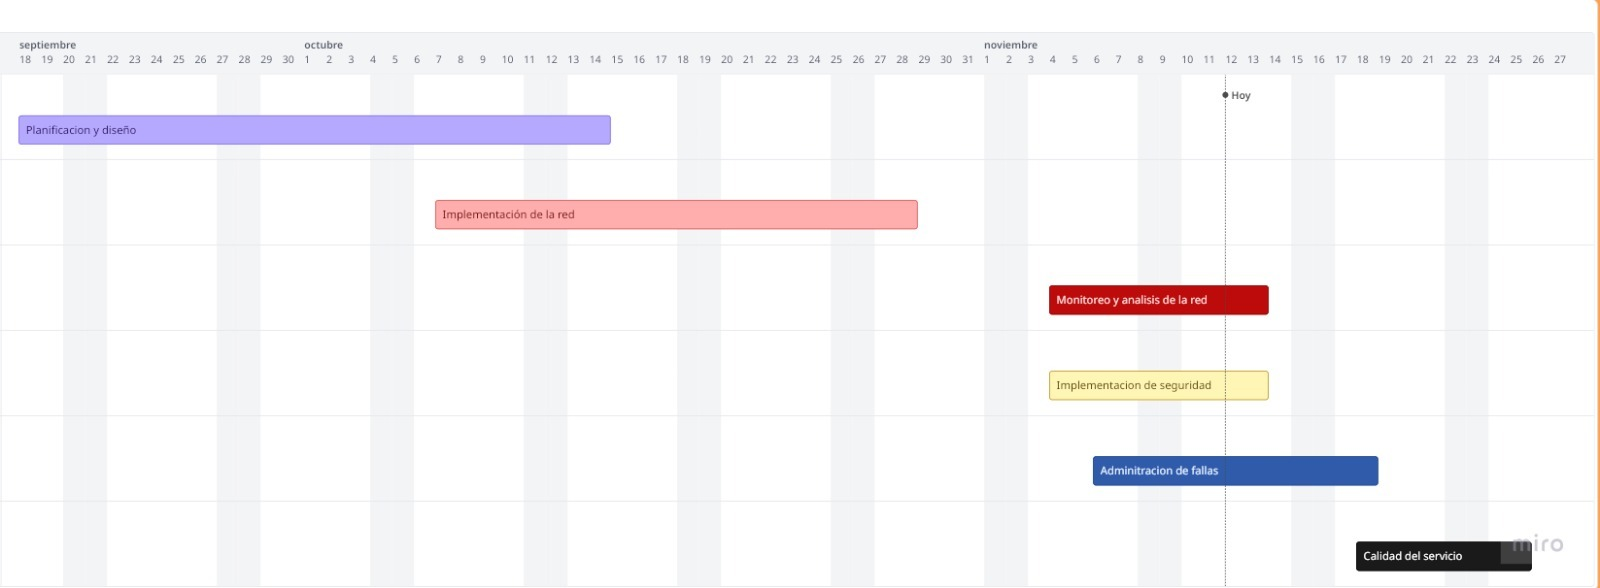
\includegraphics[width=\linewidth]{../images/cronograma.jpg}
	\caption{Cronograma de actividades (18 de septiembre — 25 de noviembre).}
\label{fig:cronograma}
\end{figure}


El cronograma distribuye de manera uniforme las tareas en un horizonte temporal que abarca desde mediados de septiembre hasta finales de noviembre. Permite coordinar los esfuerzos del equipo, identificar dependencias y monitorear el progreso del proyecto.

La asignación de tiempos para las seis fases del proyecto se detalla a continuación:

\begin{enumerate}
	\item Planificación y diseño

			\textbf{Tiempo:} Del 18 de septiembre al 14 de octubre.

			\textbf{Propósito:} Esta será la fase fundamental donde se definirá la arquitectura completa de la red, se seleccionará la tecnología y el hardware, y se establecerán los objetivos del proyecto.

	\item Implementación de la red

			\textbf{Tiempo:} Del 7 de octubre al 28 de octubre.

			\textbf{Propósito:} Instalación física del cableado, switches, routers y puntos de acceso, y configuración de la conectividad básica.

	\item Monitoreo y análisis de la red

			\textbf{Tiempo:} Del 4 de noviembre al 13 de noviembre.

			\textbf{Propósito:} Vigilar el rendimiento, identificar cuellos de botella y analizar el tráfico mediante herramientas de monitoreo.

	\item Implementación de seguridad

			\textbf{Tiempo:} Del 4 de noviembre al 13 de noviembre.

			\textbf{Propósito:} Configurar firewalls, políticas de acceso, sistemas de detección de intrusos y asegurar las conexiones.

	\item Administración de fallas

			\textbf{Tiempo:} Del 6 de noviembre al 18 de noviembre.

			\textbf{Propósito:} Establecer procesos de detección, diagnóstico y resolución de fallas para minimizar el impacto.

	\item Calidad del servicio (QoS)

			\textbf{Tiempo:} Del 18 de noviembre al 25 de noviembre.

			\textbf{Propósito:} Implementar políticas de Calidad de Servicio para priorizar tráfico crítico (por ejemplo, videollamadas) y garantizar el rendimiento de aplicaciones importantes.
\end{enumerate}





